\section{Newton's Method}\index{Newton's method}
\label{sec:newtons_method}

\subsection*{Recommended Tutorials:}
\begin{itemize}[noitemsep]
	\item \nameref{chp:derivative}, pg. \pageref{chp:derivative}
	\item \nameref{chp:conditional_statements_and_loops}, pg. \pageref{chp:conditional_statements_and_loops}
\end{itemize}

\subsection*{Introduction:}

Newton's method is an algorithm that can be used to approximate the root of a continuous function. In class, we learned that the linear approximation for $f(x)$ at $x=a$ is given by the function
\marginnote{There are some practical considerations you should be aware of when using Newton's method including: 
\begin{enumerate}
\item how difficult it is to compute the derivative, 
\item poor initial guesses, and 
\item convergence to the wrong root.  
\end{enumerate} 
Any of these will lead Newton's method to be less useful.}
\[ L(x) = f'(a) (x-a) + f(a). \] \index{Newton's method!formula}
Now, suppose we are given a continuous function $f$ with a root $r$ and wish to approximate $r$. One way we could do this is to choose a value $a$ close to $r$, determine the linear approximation $L(x)$ at $x=a$ and find the root of $L(x)$ by setting it to zero:
\[ f'(a) (x-a) + f(a) = 0 .\]
This gives the root of $L(x)$ as
\marginnote{Newton's method will fail for a number of different reasons:
\begin{enumerate}
\item if the starting point leads to a cycle between two or more points, \item if the iteration point is at a critical point, or 
\item if the derivative is discontinuous.
\end{enumerate}   
Be careful of such situations.}
\[ x = a - \frac{f(a)}{f'(a)}. \]
Now, assuming that this value of $x$ is closer to $r$ than our initial value $a$, we could repeat this process again. Therefore, our formula for each new approximation can be simplified to \[x_{new} = x_{old} - \dfrac{f(x_{old})}{f^{\prime}(x_{old})}.\]  By repeated evaluation of this equation, we can continue to find better approximations of $r$.

\begin{figure}[h]
\label{fig:newtonsmethod}
\centering
\caption{Using three iterations of Newton's Method to approximate the root $r$.}
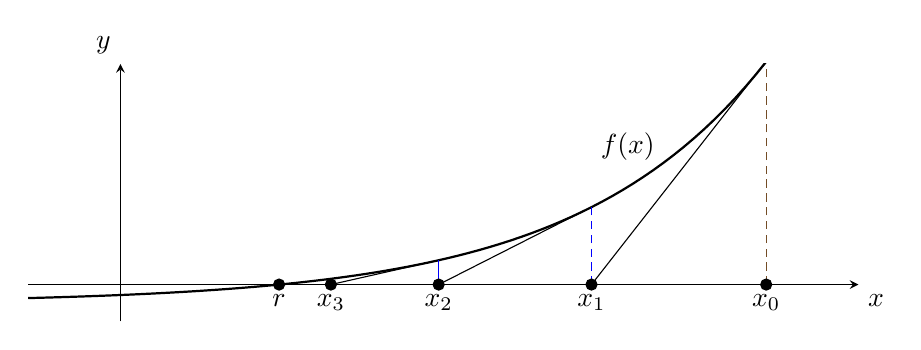
\begin{tikzpicture}
\begin{axis}[
	width=\linewidth,
	height=0.4\linewidth,
	axis lines=middle,
	xlabel={$x$},
	ylabel={$y$},
	xlabel style={below right},
	ylabel style={above left},
	xmin=-10, xmax=80, xtick={0},
	ymin=-20, ymax=120, ytick={0}
]
	\addplot [domain=-10:100, samples=100, thick] {1.05^(x+30)-10};
	\addplot [domain=51.06267696:70, samples=100] {6.415967957*x-327.6164992};
	\addplot [domain=34.49325000:51.06267696, samples=100] {2.546792633*x-87.84715498};
	\addplot [domain=22.80985278:34.49325000, samples=100] {1.134746996*x-25.88341192};
	\addplot[mark=*] coordinates {(17.19363282,0)} node [below] {$r$};
	\addplot[mark=*] coordinates {(70,0)} node [below] {$x_0$};
	\addplot +[mark=none] coordinates {(70,0) (70, 121.5012578)};
	\addplot[mark=*] coordinates {(51.06267696,0)} node [below] {$x_1$};
	\addplot +[mark=none] coordinates {(51.062676960,0) (51.06267696, 42.19889452)};
	\addplot[mark=*] coordinates {(34.49325000,0)} node [below] {$x_2$};
	\addplot +[mark=none] coordinates {(34.49325000,0) (34.49325000, 13.25769989)};
	\addplot[mark=*] coordinates {(22.80985278,0)} node [below] {$x_3$};
	\addplot +[mark=none] coordinates {(22.80985278,0) (22.80985278, 3.15236232)};
	\draw(axis cs:55,75) node {$f(x)$};
\end{axis}
\end{tikzpicture}
\end{figure}
\marginnote[-1.3cm]{Newton's method can be used to approximate the critical points (max or min) of a function.  Since a function $f$ has a maximum or minimum at a point $c$ for which $f^{\prime}(c) = 0$, we can simply change our Newton's method to be \[x_{new} = x_{old} - \dfrac{f^{\prime}(x_{old})}{f^{\prime \prime}(x_{old})}.\]}
In the following exercises, you can make use of the \texttt{NewtonsMethod()} command, provided as part of the \texttt{Student[Calculus1]} package. A useful example can be found in Tutorial \ref{sec:newtonsmethod} on page \pageref{sec:newtonsmethod}. However, it is also beneficial to try more advanced coding methods and implement a ``while" loop if you are interested; information regarding loops is given in Tutorial \ref{chp:conditional_statements_and_loops} on page \pageref{chp:conditional_statements_and_loops}.
\marginnote[-0.5cm]{To load the \texttt{Student[Calculus1]} package, the \texttt{with()} command needs to be used. Make sure you capitalize the appropriate letters in the package name, or else it will not load the necessary commands.}


\subsection*{Exercises:}

\begin{enumerate}
\marginnote[0.2cm]{Be sure to load the \texttt{Student[Calculus1]} package before using the \texttt{NewtonsMethod()} command. The package only needs to be loaded once in your document, not every time you use one of its commands.}\index{Newton's method!NewtonsMethod}
    \item  Use Maple's \texttt{NewtonsMethod()} command to determine the value of the root of the function $f(x) = x^2 - 2$.  Use an initial guess of $2$.  Iterate until you get $10$ decimal places of accuracy.
    \marginnote[0.4cm]{Adding the optional \texttt{iterations} parameter to the \texttt{NewtonsMethod()} command allows you to choose how many iterations are performed. By default, \texttt{NewtonsMethod()} carries out $5$ iterations.}
    
    \marginnote[0.4cm]{The output of Maple's \texttt{NewtonsMethod()} command can be displayed in different ways, depending on whether the \texttt{output} parameter is set equal to \texttt{value}, \texttt{plot}, \texttt{animation}, or \texttt{sequence}. See page \pageref{sec:newtonsmethod} for more information.}
    \item   Apply Newton's method to determine the value of the root of the function $f(x) = x^2 - 2$.  Use an initial guess of $-2$.  Iterate until you get $10$ decimal places of accuracy.
    \item   We cannot use Newton's method to find the root of the function $f(x) = x^2 - 2$ if we use an initial guess of $0$.  Use a graph to help explain why, and discuss your answer by using a new paragraph.
    \item   Suppose you wish to find the value of $\sqrt{7}$ using Newton's method.
	    \begin{enumerate}
	    \item What function would we use if we wanted to apply Newton's method to determine the value of $\sqrt{7}$? State your answer using a new paragraph.
	    \item Evaluate $\sqrt{7}$ to $15$ digits using \texttt{evalf()}. Apply Newton's method to the function from part (a) with an appropriate initial guess for $x$ and verify that the values agree.
	    \end{enumerate}
    \item   Newton's method converges with \textit{quadratic convergence}.  That roughly means that you will get twice as many correct digits for $x_{new}$ as you did for $x_{old}$. Iterate Newton's method for \[g(x) = x^2 - \sin(x) - 0.5\] with an initial guess of $x = 2$.  Find the value of the zero of $g(x)$ to $16$ decimal places.
    
   \item (Optional) Write a "while" loop that allows you to solve exercises 1 and 2.\index{loops}
\end{enumerate}